% !TEX root = /Users/kquine/Dropbox/Research/Papers/2015/CPS-SMT-RTSS/cps-rtss.tex

%
\section{Case Studies}
\label{sec:case-studies}

This section presents
four case studies for SMT-based analysis of 
networks of hybrid systems.
%networked thermostats,
%networked water tank controllers,
%and distributed controllers for smoothly turning an airplane.
%
These case studies involve nontrivial (nonlinear) ODEs,
because of continuous physical interaction between components.
%
We have implemented our techniques in the dReal SMT solver, and 
performed formal analysis for these three case studies using the tool.
%The dReal tool is
%built on the general DPLL($\mathcal{T}$) framework,
%with underlying theory solvers for the real numbers and ODEs 
%based on the ICP (interval constraint propagation) procedure \cite{dreal}.
%\marginpar{\textbf{Sean, could you write some  implementation details if necessary?}}
%
We have compared the performance of  the new encoding
with the standard encoding,
and with the existing heuristics used in the dReach tool \cite{dReach},
which
\emph{explicitly enumerates} all paths in the mode graph of a hybrid automaton
and generates many small SMT formulas.
%
%We have also compared the performance with the \texttt{flow*} tool \cite{flowstar}.
All the experiments %in this section
were conducted on Intel Xeon 2.0 GHz with 64 GB memory.
%running 64-bit Ubuntu 12.04.5 LTS.



We have applied our techniques to 
design and verify two  multirate distributed cyber physical systems:
a distributed control system for turning an airplane where its effectors located 
in the airplane's wings (Section~\ref{sec:airplane}),
and a robotics system with  a conveyer belt and robot arms
for physically simulating a Turing machine (Section~\ref{sec:turing-machine}).
%
Both systems are  distributed \emph{hybrid} systems
consisting of \emph{discrete} multirate periodic controllers, interconnected by a wired network,
and 
interacting with their \emph{continuous} local environments.
The systems can provide PALS bounds $\Gamma$;
%\begin{inparaenum}[(i)]
%\item 
in particular, 
a bound $\epsilon > 0$ on the imprecisions of the local clocks.
%of the components.
%\item minimum and maximum message transmission times 	
%%$0 \leq \mu_{\min} \leq \mu_{\max}$
%between two different components, 		
%and
%\item minimum and maximum execution times 	
%%$0 \leq \alpha_{\min} \leq \alpha_{\max}$ 
%to perform transitions of any component.
%\end{inparaenum}
%
Therefore, using Multirate PALS,
the discrete behavior can be precisely modeled 
as a multirate synchronous system $\mathcal{E}$.
However, the continuous behavior
still depends on the exact values of the local clocks,
given by clock synchronization mechanisms.
The local physical environments of different components 
can be simultaneously correlated to each other,
which cannot be modeled as network communications in general.
The hybrid system modeling framework in Section~\ref{sec:env-const}
was shown to be effective for dealing with these difficulties.
The bounded model checking method in Section~\ref{sec:formula}
was applied to verify
the  given safety properties of the systems,
with respect to (bounded) real number parameters and inputs,
by means of \texttt{dReal}-based SMT solving in Section~\ref{sec:formula}.






\subsection{Turning an Airplane}
\label{sec:airplane}
..

(adapted from \cite{ftscs-journal}),


We consider a networked control system
to perform the turning maneuver of an airplane,
adapted from \cite{ftscs-journal},
in which a main controller directs subcontrollers for the ailerons and the rudder.
%
To make a turn,
an aircraft rolls %towards the direction of the turn
by moving its ailerons (surfaces attached to the end of the wings),
while its rudder (a surface attached to the vertical tail)
is used to counter adverse yaw
(a yawing moment %in the opposite direction 
caused by the rolling).
%
The lateral dynamics of an aircraft
can be specified as nonlinear differential equations
\cite{stevens2003aircraft}:
\[
\begin{aligned}
\dot{\beta} &= Y(\beta,\delta_a,\delta_r) / m V - r + V / g * \cos(\beta) * \sin(\phi)
&
\dot{\phi} &= p
\\
\dot{p} &= (c_1 r + c_2 p)\cdot r \cdot \tan(\phi) + c_3 L(\beta,\delta_a,\delta_r) + c_4 N(\beta,\delta_a,\delta_r)
&
\dot{\psi} &= g / V \tan(\phi)
\\
\dot{r} &= (c_8 p - c_2 r) \cdot r \cdot \tan(\phi) + c_4 L(\beta,\delta_a,\delta_r) + c_9 N(\beta,\delta_a,\delta_r)
\end{aligned}
\]
with:
\begin{inparaenum}[(i)]
	\item  state variables $\beta$ for the yaw angle, 
        $p$ for the rolling moment,
        $r$ for the yawing moment,
        $\phi$ for the roll angle, 
        and $\psi$ for the direction,
	\item control variables $\delta_a$ for the angle of the ailerons,
	and $\delta_r$ for the angle of the rudder,
	and
	\item 
	linear functions  
	$Y(\beta,\delta_a,\delta_r)$, $L(\beta,\delta_a,\delta_r)$, and $N(\beta,\delta_a,\delta_r)$
	to denote 
	side force, rolling moment, and yawing moment of the airplane.
%	\item constants $V$ for the airplane's velocity,
%		$g$ for the standard gravity, 
%		and 
%		$Y_\beta, Y_{\delta_r}, 
%		L_\beta, L_p, L_r, L_{\delta_a}, L_{\delta_r},
%		N_\beta, N_p, N_r, N_{\delta_a}, N_{\delta_r}$
%		determined by the shape and status of the airplane.
\end{inparaenum}
%
The main controller has one mode,
and determines the desired control angles. % for each period.
The two subcontroller have two modes for moving up or down their surfaces,
and gradually change the surface angles according to the main controller.
%
We consider three variants of this model:
a single-rate nonlinear model
in which every controller has a $0.5$ period,
%and involves a shared timer variable $\tau$ with the flow condition $\dot{\tau} = 1$.
an approximated linear model
assuming small perturbations given by linear differential equations \cite{allerton2009principles}, and
a multirate linear model 
in which
the aileron controller has a $0.25$ period and the rudder controller has a $0.5/3$ period.


%\[
%\left[\begin{array}{c}
%\dot{\beta}\\\dot{p}\\\dot{r}\\\dot{\phi}\\\dot{\psi}
%\end{array}\right]
%=
%\left[\begin{array}{ccccc}
%Y_\beta & 0 & -1 & (g/V) & 0\\
%L_\beta & L_p & L_r & 0 & 0\\
%N_\beta & N_p & N_r & 0 & 0\\
%0 & 1 & 0 & 0 & 0\\
%0 & 0 & 0 & (g/V) & 0
%\end{array}\right]
%\left[\begin{array}{c}
%{\beta}\\{p}\\{r}\\{\phi}\\{\psi}
%\end{array}\right]
%+
%\left[\begin{array}{cc}
%0 & Y_{\delta_r}\\
%L_{\delta_a} & L_{\delta_r}\\
%N_{\delta_a} & N_{\delta_r}\\
%0 & 0 \\
%0 & 0
%\end{array}\right]
%\left[\begin{array}{c}
%\delta_a\\ \delta_r
%\end{array}\right]
%\]




\subsection{Quadrotor Attitude Controller}
\label{sec:quadrotor}
..




\subsection{Steam Boiler Controller}

...

\subsection{Networked Water Tank Controllers.}

A number of water tanks are connected by pipes as shown in Figure~\ref{fig:water}.
The water level in each tank is separately controlled by the pump in the tank
(adapted from \cite{kowalewski1999case,raisch1999approximating}).
Similarly, each water level depends on the pump's mode $m \in \{m_\texttt{on}, m_\texttt{off}\}$
and the levels of the adjacent tanks.
The water level $x_i$ of tank $i$ changes according to the differential equations:
\[
\begin{aligned}
A_i \dot{x}_i &=  (q_i + a \sqrt{2g} \sqrt{x_{i-1}})  - a \sqrt{2g} \sqrt{x_i}
&& \mbox{if}\;\; m_i = m_\texttt{on},
\\
A_i \dot{x}_i &= a \sqrt{2g} \sqrt{x_{i-1}}  - a \sqrt{2g} \sqrt{x_i}
&& \mbox{if}\;\; m_i = m_\texttt{off},
\end{aligned}
\]
where $A_i, q_i, a $ are constants determined by the size of the tank, the power of the pump, 
and the width of the pipe,
and $g$ is the standard gravity constant ($x_0 = 0$ for the leftmost tank $1$).
%
There is also a shared timer variable $\tau$ 
with the flow condition $\dot{\tau} = 1$.
Every pipe controller synchronously performs its discrete transitions:
for each second, 
the pump is on if $x_i \leq L_{\min}$, and off if $x_i > L_{\max}$.

%We consider the cases of networks of two and three water tanks
%with the parameters
%$a = 0.5$,
%$g = 9.8$,
%$A_1 = 2$, 
%$A_2 = 4$, 
%$A_3 = 3$, 
%$q_1 = 5$,
%$q_2 = 3$,
%$q_3 = 4$,
%$L_{\min} = L_{\max} = 5$,
%and the initial condition $\wedge_{i} 4.9 < x_i < 5.1$.
%We have performed bounded model checking up to $k = 5$
%for the properties $\mathit{safe} = \wedge_{i} 4.9 < x_i < 5.1$ 
%and $\mathit{safe} = \wedge_{i} 19 < x_i < 21$.
%We have performed 
%inductive analysis 
%to verify that the property $\mathit{safe} = \wedge_{i} 1 < x_i < 9$
%holds at the end $\tau > 0.99$ of each period.


\begin{figure}[t]
\centering
%
\begin{minipage}[t]{.5\textwidth}
\centering
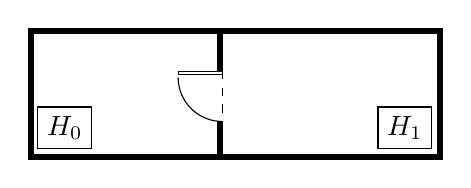
\begin{tikzpicture}[scale=0.8] %baseline=(current bounding box.north)
%room1
\filldraw (0,-0.6) rectangle  + (-0.08,0.6)
	(0,0) rectangle  + (-3,0.08)
	(-3,0.08) rectangle  + (-0.08,-2.0)
	(-3.08,-2.0) rectangle  + (3,0.08)
	(0,-2.0) rectangle  + (-0.08,0.6);
\path (-2.5,-1.5) node[draw] { $H_0$};
\draw[dashed] (0,-0.6) -- (0,-2);
%room2
\filldraw (0,0) rectangle  + (3.5,0.08)
	(3.5,0.08) rectangle  + (-0.08,-2.0)
	(3.5,-2.0) rectangle  + (-3.5,0.08);
\path (2.9,-1.5) node[draw] (m2){ $H_1$};
%door
\draw (0,-0.6) rectangle +(-0.7,-0.05);
\draw (-0.7,-0.7) arc (180:270:0.7);
\end{tikzpicture}
\caption{Two interconnected rooms. %  by an open door.
} \label{fig:adj-rooms}
\end{minipage}%
\begin{minipage}[t]{.5\textwidth}
\centering
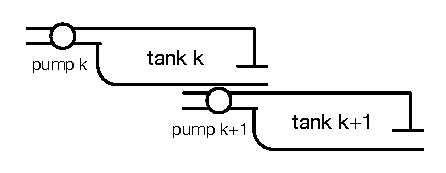
\includegraphics[clip=true,trim=0.3cm 0.35cm 0.3cm 0.35cm,width=0.9\columnwidth]{water.pdf}    
\caption{Two connected water tanks}  \label{fig:water}
\end{minipage}
\end{figure}





\subsection{Networked Thermostat Controllers.}

A network of classical thermostat hybrid automata is considered 
(where the specification of a single hybrid automaton is adapted from \cite{henzinger2000theory}). 
A number of rooms are interconnected by open doors,
and the temperature of each room is separately controlled by each thermostat
that turns its heater on and off.
(e.g., Figure~\ref{fig:adj-rooms}  for the case of two rooms).
The temperature of each room depends on
the heater's mode $m \in \{m_\texttt{on}, m_\texttt{off}\}$  and the temperatures of the other rooms.
E.g., for three rooms $I = \{0,1,2\}$, 
the temperature $x_i$ of room $i \in I$
changes according to the differential equations:
\[
\begin{aligned}
\dot{x}_i &= K_i \big(h_i - ((1- \textstyle\sum_{j \in I \setminus \{i\}} k_{i,j}) x_0 + \sum_{j \in I \setminus \{i\}} k_{i,j}  x_j)\big)
&& \mbox{if}\;\; m_i = m_\texttt{on},
\\
\dot{x}_i &= - K_i \big((1- \textstyle\sum_{j \in I \setminus \{i\}} k_{i,j}) x_0 + \sum_{j \in I \setminus \{i\}} k_{i,j}  x_j\big)
&& \mbox{if}\;\; m_i = m_\texttt{off},
\end{aligned}
\]
where $K_i, h_i \in \mathbb{R}$ are constants depending on
the size of room $i$ and the heater's power, respectively,
and $k_{i,j} \in \mathbb{R}$ is determined by the size of the open door between rooms $i$ and $j$.
%
Every thermostat controller synchronously performs its discrete transitions.
For each second, 
the heater is turned on if $x_i \leq T_{\min}$,
and turned off if $x_i > T_{\max}$.
To keep track of each one-second period,
every automaton has a \emph{shared} timer variable $\tau$ 
with the flow condition $\dot{\tau} = 1$.

%We consider the cases of networks of two and three thermostats
%with the parameters
%$K_1 = 0.015$, 
%$K_2 = 0.045$, 
%$K_3 = 0.03$, 
%$h_1 = 100$,
%$h_2 = 200$,
%$h_3 = 300$,
%$k_{1,2} = k_{2,1} = 0.01$,
%$k_{2,3} = k_{3,2} = 0.05$,
%$k_{1,3} = k_{3,1} = 0.02$,
%$T_{\min} = T_{\max} = 20$,
%and the initial condition $\wedge_{i} 19 < x_i < 21$.
%We have performed bounded model checking up to $k = 5$
%for $\mathit{safe} = \wedge_{i} 15 < x_i < 25$ 
%(the reachability of $\neg\mathit{safe}$ unsat)
%and $\mathit{safe} = \wedge_{i} 19 < x_i < 21$ 
%(the reachability of $\neg\mathit{safe}$ sat).
%We have also performed 
%inductive analysis 
%to verify that the property $\mathit{safe} = \wedge_{i} 11 < x_i < 29$
%holds at the end $\tau > 0.99$ of each period.


%The parallel composition
%is the hybrid automaton
%$H_1 \parallel H_2 = (X, Q, \{\alpha\}, \mathit{init}, \mathit{inv}, \mathit{flow}_i, \mathit{jump}_i)$, where:
%\begin{itemize}
%	\item $X = \{x_0, x_1, \tau\}$, with the shared timer variable $\tau$,
%	\item $Q = \{(m_0, m_1) \mid m_0, m_1 \in \{m_\texttt{on}, m_\texttt{off}\}\}$,
%	\item $\mathit{init} = \{((m_0,m_1), (v_0, v_1, 0)) \in Q \times \mathbb{R}^3 \mid 19 < x_0, x_1 < 21 \}
%	\item $\mathit{inv}(m_0,m_1) = \{(v_0, v_1, t) \in \mathbb{R}^3 \mid 0 \leq t \leq 1\}$,
%	\item $(f_0, f_1, f_\tau) \in \mathit{flow}(m_0, m_1)$ iff 
%	for $i = 0,1$,
%	$\dot{f_i} = \mathit{flow}_\texttt{on}^i(x_i, x_{1-1})$
%	if $m_i = m_\texttt{on}$,
%	$\dot{f_i} = \mathit{flow}_\texttt{off}^i(x_i, x_{1-1})$
%	if $m_i = m_\texttt{off}$, 
%	and 	$\dot{f_\tau} = 1$, and
%	\item $((m_1,m_1), (v_0, v_1, 1)) \xrightarrow{\alpha} ((m_1',m_2'), (v_0, v_1, 0)) \in \mathit{jump}$ 
%	holds, where
%	for each $i \in \{0,1\}$,
%	$m_i' = \ite{v_i \leq 20}{m_\texttt{on}}{m_\texttt{off}}$.
%\end{itemize}


\subsection{Automated Highway System}


...

